% Workflow figure only: landscape.
\chapstart
\section{PHÂN TÍCH VÀ THIẾT KẾ HỆ THỐNG}
\subsection{Tác nhân và yêu cầu chức năng}
BroomSharing tổ chức nghiệp vụ theo ba tác nhân: người thuê, Host và Admin. Người thuê tìm kiếm và gửi yêu cầu sử dụng không gian; Host quản lý tài sản và xử lý lượt thuê; Admin kiểm duyệt và giải quyết các trường hợp vượt quyền của hai bên. Các yêu cầu chức năng được nhóm theo trách nhiệm tại Bảng~\ref{tab:ch2-actors}.

\begin{table}[!htbp]\centering\small
\caption{Tác nhân và phạm vi chức năng}\label{tab:ch2-actors}
\begin{tabularx}{\textwidth}{@{}p{2cm}X@{}}\toprule
Tác nhân & Chức năng chính\\\midrule
Người thuê & Quản lý tài khoản; tìm, lọc và xem phòng trên bản đồ; lưu yêu thích; đặt, hủy và theo dõi booking; thanh toán; chat; đánh giá và báo cáo vi phạm; gửi đơn làm Host.\\
Host & Quản lý tòa nhà và phòng; thiết lập giá, lịch; gửi xét duyệt và mở cho thuê; xử lý booking, nhận phòng, hoàn tất hoặc ghi nhận không đến; gửi minh chứng và phản hồi báo cáo. Host vẫn có thể thuê phòng của người khác.\\
Admin & Duyệt đơn Host, minh chứng và bài đăng; đình chỉ phòng, khóa Host; xử lý báo cáo, booking của Host bị khóa; xác minh việc sử dụng, đối soát lịch giữ chỗ và tra cứu nhật ký.\\\bottomrule
\end{tabularx}
\end{table}

Host là vai trò có thêm quyền cho thuê sau khi hồ sơ được duyệt. Quyền Host không đồng nghĩa bài đăng được công bố ngay: từng phòng còn phải qua xét duyệt và được chủ phòng mở cho thuê. Dịch vụ thanh toán là tác nhân bên ngoài, tiếp nhận giao dịch và trả kết quả cho hệ thống.

\subsection{Sơ đồ công việc}
\subsubsection{Đăng ký Host và công bố không gian}
Người dùng gửi đơn làm Host kèm thông tin và hai ảnh giấy tờ DEMO. Admin xem hồ sơ trước khi chấp thuận hoặc từ chối. Khi được cấp quyền, Host tạo tòa nhà, bổ sung phòng, cấu hình giá, lịch và gửi bài đăng xét duyệt. Phòng chỉ xuất hiện trong danh sách cho thuê khi vừa được duyệt vừa ở trạng thái hoạt động. Luồng tại Hình~\ref{fig:app-host-workflow} tách riêng quyết định cấp quyền Host và quyết định duyệt phòng.

\subsubsection{Tạo và xử lý yêu cầu đặt chỗ}
Người thuê chọn phòng, thời gian và kiểm tra giá trước khi gửi yêu cầu. Hệ thống kiểm tra trạng thái phòng, quyền của các bên và lịch khả dụng; nếu hợp lệ, booking được tạo ở trạng thái \texttt{PENDING}. Booking, lịch giữ chỗ, thông tin cập nhật của phòng và nhật ký được ghi trong cùng transaction. Lịch này là phần giữ chỗ tạm trong tối đa 5 phút, không vượt giờ bắt đầu thuê; yêu cầu khác không được chiếm cùng khoảng thời gian trong lúc giữ chỗ còn hiệu lực.

Hình~\ref{fig:ch2-booking-workflow} thể hiện các nhánh xử lý sau khi tạo yêu cầu. Ứng dụng mở QR ngay sau bước tạo booking. Backend ghi nhận đủ 40\% đúng hạn mới chuyển booking sang \texttt{CONFIRMED}; Host không duyệt booking mới. Khi hết hạn hoặc hủy, backend đối chiếu trạng thái của payOS trước khi kết thúc link chưa trả, nhả lịch và giữ lịch sử. Nếu chưa xác định được kết quả từ nhà cung cấp, lịch chưa được nhả cho đến khi đối soát được kết quả.

\subsubsection{Sử dụng phòng và xử lý ngoại lệ}
Booking đã xác nhận được Host ghi nhận việc nhận phòng trong khoảng thời gian thuê và hoàn tất sau giờ kết thúc. Nếu khách không đến, Host ghi nhận \texttt{NO\_SHOW} sau giờ kết thúc, kèm lý do. Trường hợp đã sử dụng nhưng thiếu thao tác nhận phòng cần có xác nhận sử dụng trước khi hoàn tất; thời gian trôi qua không tự chứng minh khách đã dùng phòng.

Với Host bị khóa, Admin xử lý từng booking thay vì hủy hàng loạt. Booking chưa nhận phòng có thể bị hủy với lý do; lượt đã nhận phòng có thể kết thúc do sự cố ở trạng thái \texttt{TERMINATED}. Việc sửa kết luận không đến hoặc bổ sung xác nhận sử dụng phải có nhật ký, không nhả lịch lần thứ hai. Chỉ người thuê của booking đã khép và có xác nhận sử dụng mới được đánh giá. Quy trình chi tiết được thể hiện tại Hình~\ref{fig:app-usage-workflow}.

\subsubsection{Thanh toán khoản trả trước}
Người thuê thanh toán khoản trả trước 40\% qua QR trong phạm vi một Host và kênh payOS demo đã cấu hình. Booking đang chờ thanh toán chưa được trình bày như một lượt đặt chỗ thành công. Backend Java kiểm tra danh tính, booking và giá đã chốt trước khi tạo hoặc lấy lại mã QR của cùng một yêu cầu thanh toán. Thời hạn thanh toán tính từ lúc tạo booking trên máy chủ, tối đa 5 phút và không vượt giờ bắt đầu thuê. Quay lại hoặc tiếp tục thanh toán dùng cùng mã đơn và cùng thời hạn; thao tác này không gia hạn giữ chỗ.

Kết quả do payOS gửi qua webhook chuyển tiếp được backend kiểm tra trước khi cập nhật dữ liệu. Khi nhận đủ tiền đúng hạn và khóa lịch còn hợp lệ, backend ghi \texttt{PAID} và xác nhận booking trong transaction. Ứng dụng nhận thay đổi để cập nhật QR, bộ đếm và thông báo; thanh toán thành công không tự ghi nhận khách đã đến nhận phòng. Giao dịch cần đối soát được tách khỏi trạng thái thanh toán hợp lệ, còn hoàn tiền tự động chưa thuộc phạm vi triển khai. Hình~\ref{fig:app-payment-workflow} thể hiện các thành phần tham gia luồng này.

\clearpage
\begin{landscape}\pagestyle{empty}\BroomLandscapePagetrue
\begin{figure}[p]\centering
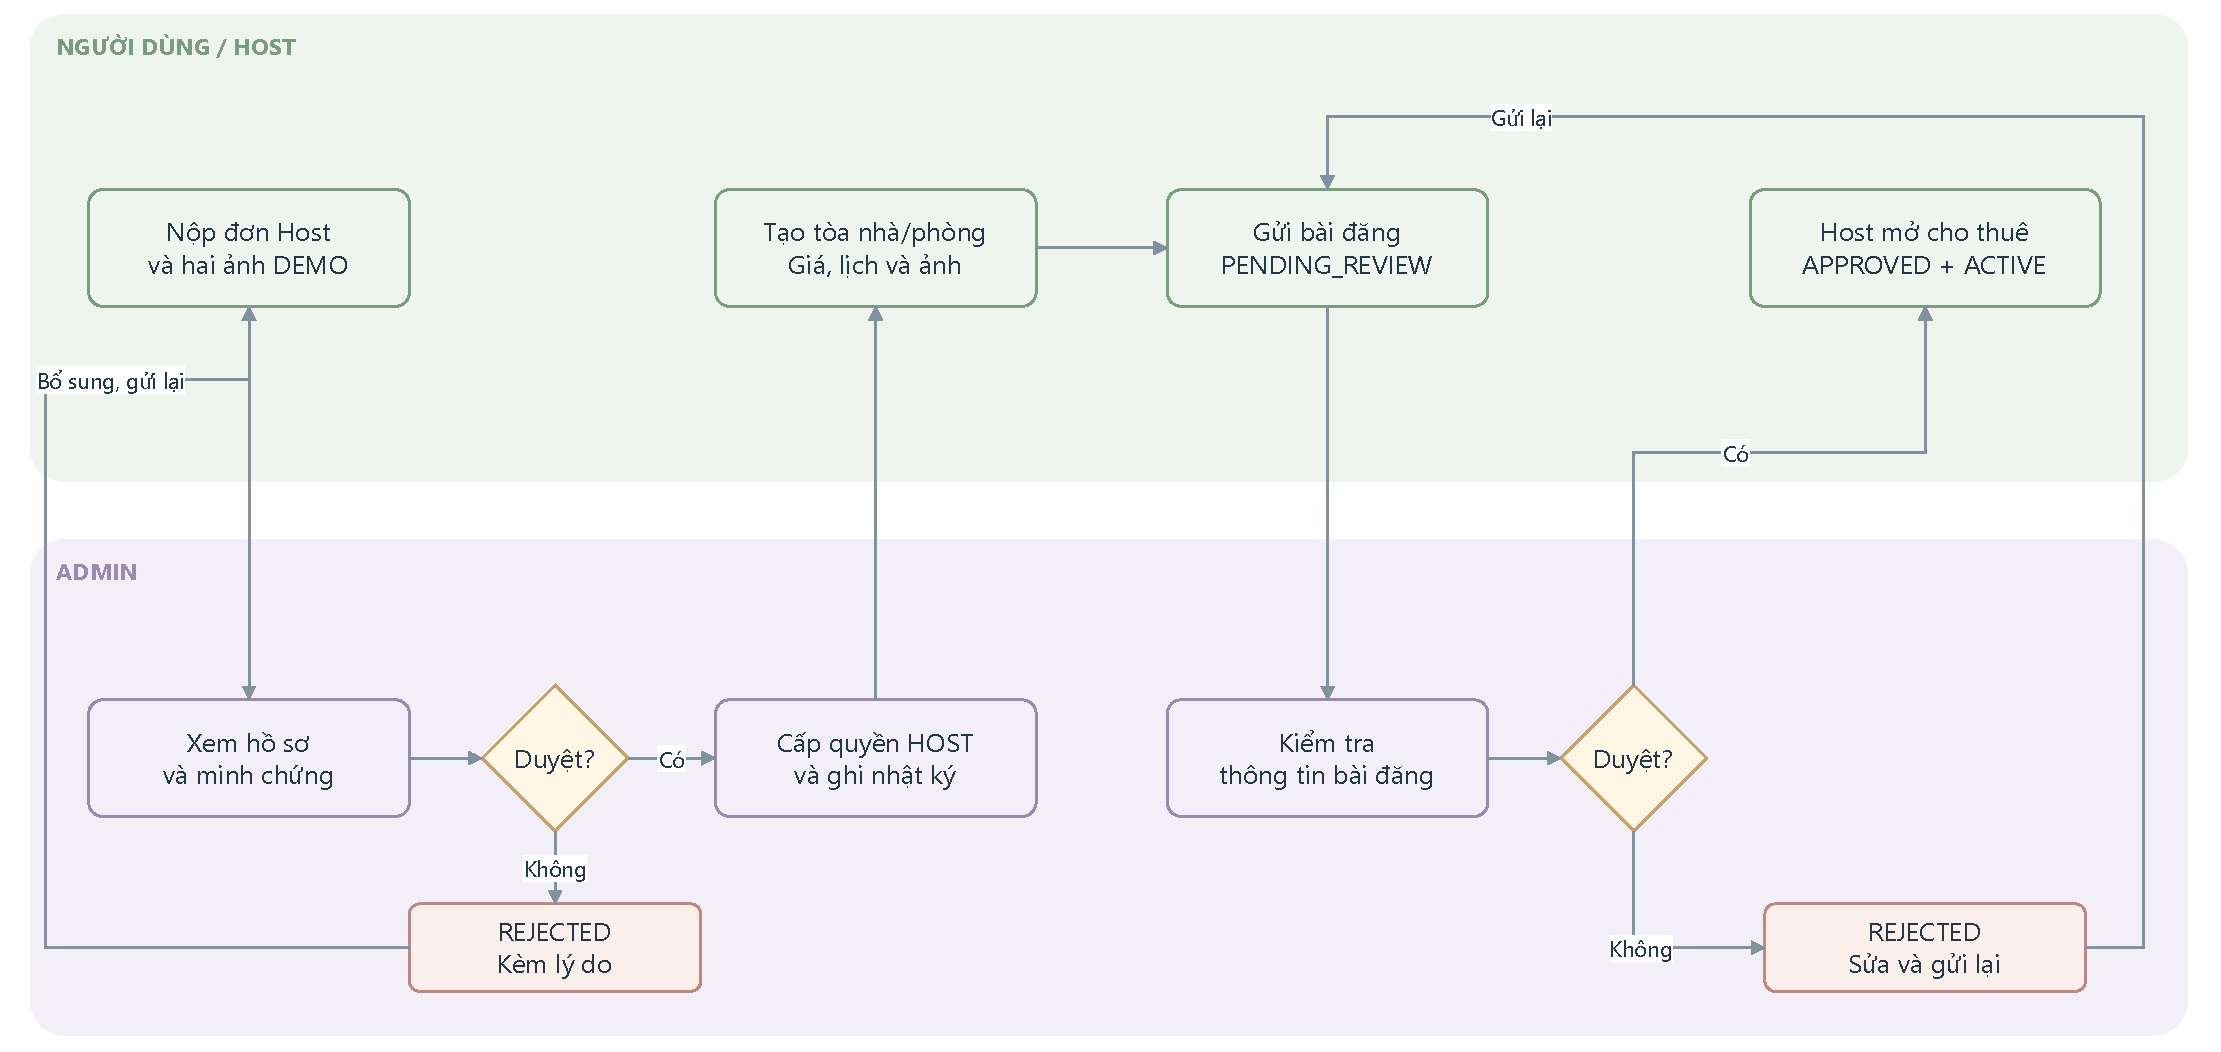
\includegraphics[page=1,width=\linewidth,height=0.82\textheight,keepaspectratio]{chapter2/workflow_diagram_v2.pdf}
\caption{Quy trình cấp quyền Host và công bố không gian.}\label{fig:app-host-workflow}
\end{figure}
\clearpage\BroomLandscapePagefalse\end{landscape}\pagestyle{fancy}
\clearpage
\begin{landscape}\pagestyle{empty}\BroomLandscapePagetrue
\begin{figure}[p]\centering
\includegraphics[page=2,width=\linewidth,height=0.82\textheight,keepaspectratio]{chapter2/workflow_diagram_v2.pdf}
\caption{Quy trình tạo, giữ lịch và xử lý yêu cầu đặt chỗ.}\label{fig:ch2-booking-workflow}
\end{figure}
\clearpage\BroomLandscapePagefalse\end{landscape}\pagestyle{fancy}
\clearpage
\begin{landscape}\pagestyle{empty}\BroomLandscapePagetrue
\begin{figure}[p]\centering
\includegraphics[page=3,width=\linewidth,height=0.82\textheight,keepaspectratio]{chapter2/workflow_diagram_v2.pdf}
\caption{Quy trình sử dụng phòng, khép lượt thuê và xác minh ngoại lệ.}\label{fig:app-usage-workflow}
\end{figure}
\clearpage\BroomLandscapePagefalse\end{landscape}\pagestyle{fancy}
\clearpage
\begin{landscape}\pagestyle{empty}\BroomLandscapePagetrue
\begin{figure}[p]\centering
\includegraphics[page=4,width=\linewidth,height=0.82\textheight,keepaspectratio]{chapter2/workflow_diagram_v2.pdf}
\caption{Luồng tạo QR và cập nhật kết quả thanh toán payOS.}\label{fig:app-payment-workflow}
\end{figure}
\clearpage\BroomLandscapePagefalse\end{landscape}\pagestyle{fancy}

\subsection{Sơ đồ phân rã chức năng}
Các chức năng được phân rã từ mục tiêu của từng vai trò đến nhóm thao tác liên quan. Nhóm người thuê bao gồm tài khoản, khám phá, booking, tương tác và hồ sơ Host; nhóm Host tập trung vào phòng, lịch và vận hành lượt thuê; nhóm Admin tập trung vào xét duyệt, xử lý vi phạm và kiểm tra nghiệp vụ. Cách phân rã tại Hình~\ref{fig:ch2-functions} làm rõ trách nhiệm mà không đồng nhất mỗi màn hình với một chức năng độc lập.

\begin{figure}[H]\centering
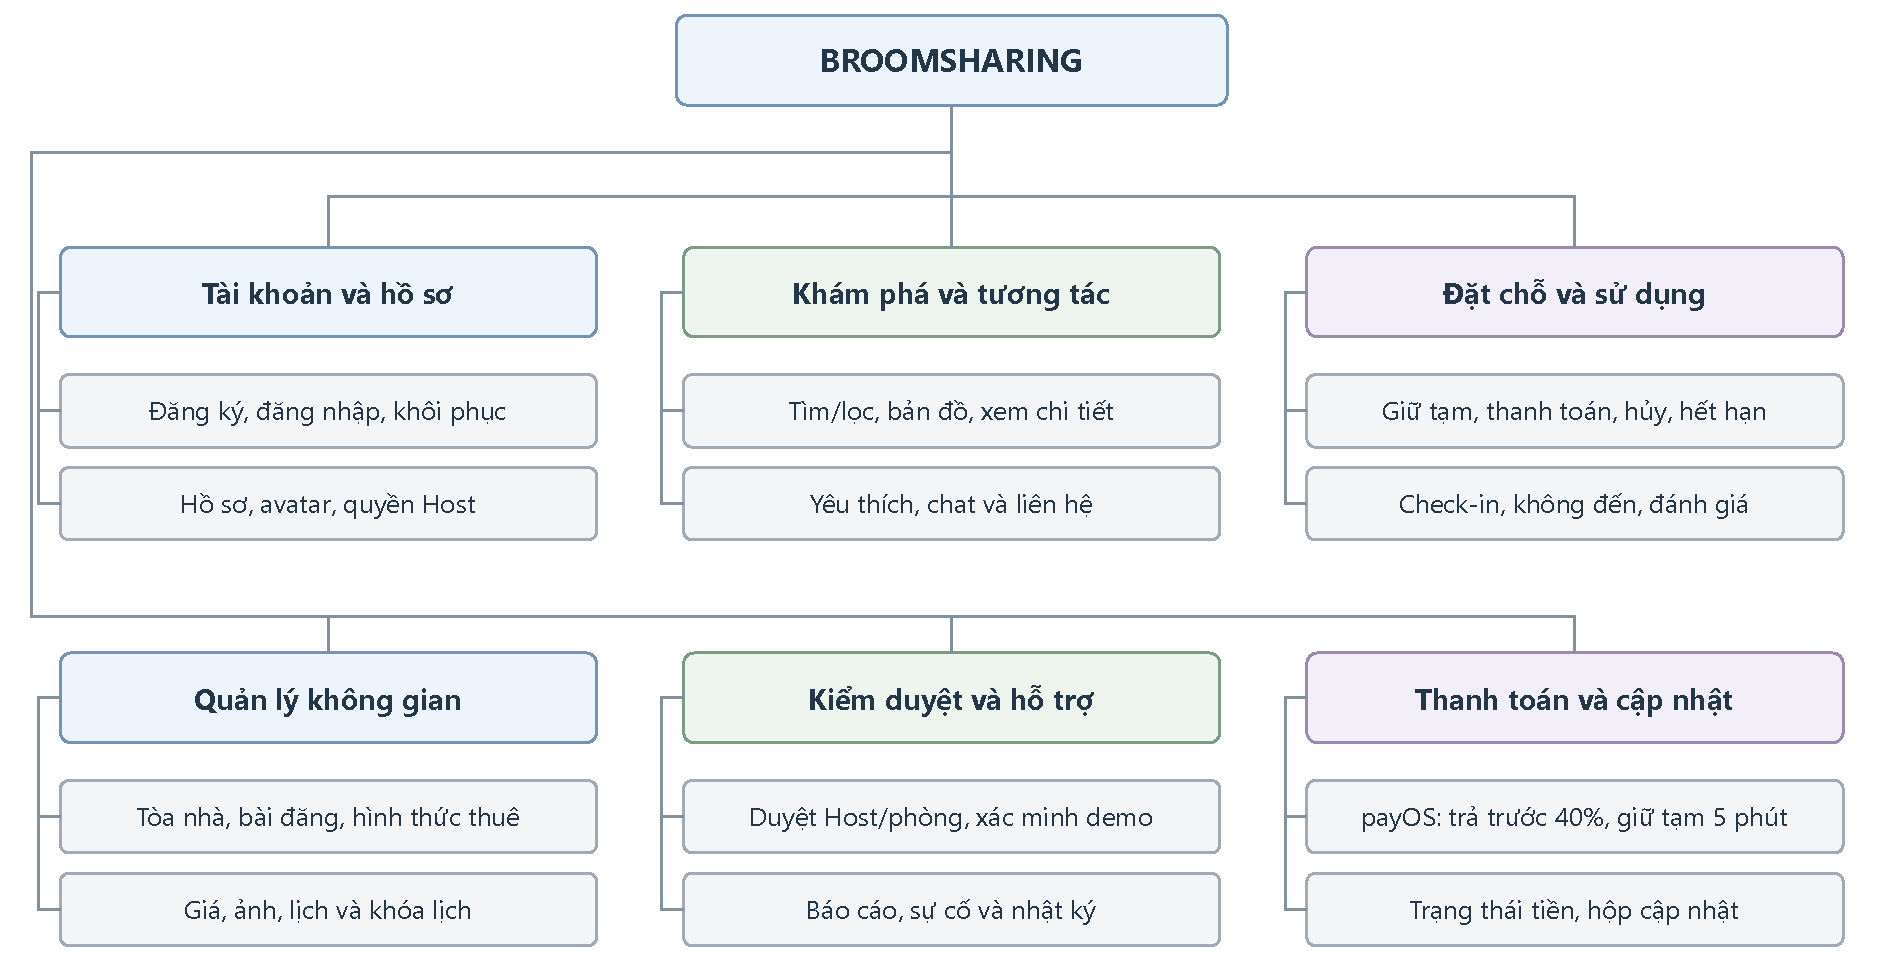
\includegraphics[page=1,width=\textwidth]{chapter2/usecase_decomposition_v2.pdf}
\caption{Phân rã chức năng tổng quát của BroomSharing.}\label{fig:ch2-functions}
\end{figure}

Chức năng tin nhắn hỗ trợ trao đổi giữa hai bên của một hội thoại. Hộp cập nhật tổng hợp sự kiện booking và trạng thái đã đọc của từng tài khoản. Đánh giá gắn với lượt đã sử dụng, còn báo cáo vi phạm được chuyển đến Admin và cho phép Host phản hồi. Các chức năng này bổ sung thông tin xử lý cho lượt thuê, đồng thời duy trì giới hạn truy cập theo vai trò và chủ thể liên quan.

Bộ phân rã chi tiết được lưu cùng tài nguyên đồ án tại \hyperref[app:project-resources]{Phụ lục C}.

\subsection{Sơ đồ use case}
Hình~\ref{fig:ch2-usecase-overview} mô tả các mục tiêu tương tác với hệ thống. Host kế thừa khả năng thuê phòng của người thuê và có thêm nhóm chức năng cho thuê. Admin có tuyến chức năng kiểm duyệt riêng; quyền quản trị không mặc định bao gồm đọc hội thoại riêng của người dùng.

\begin{figure}[H]\centering
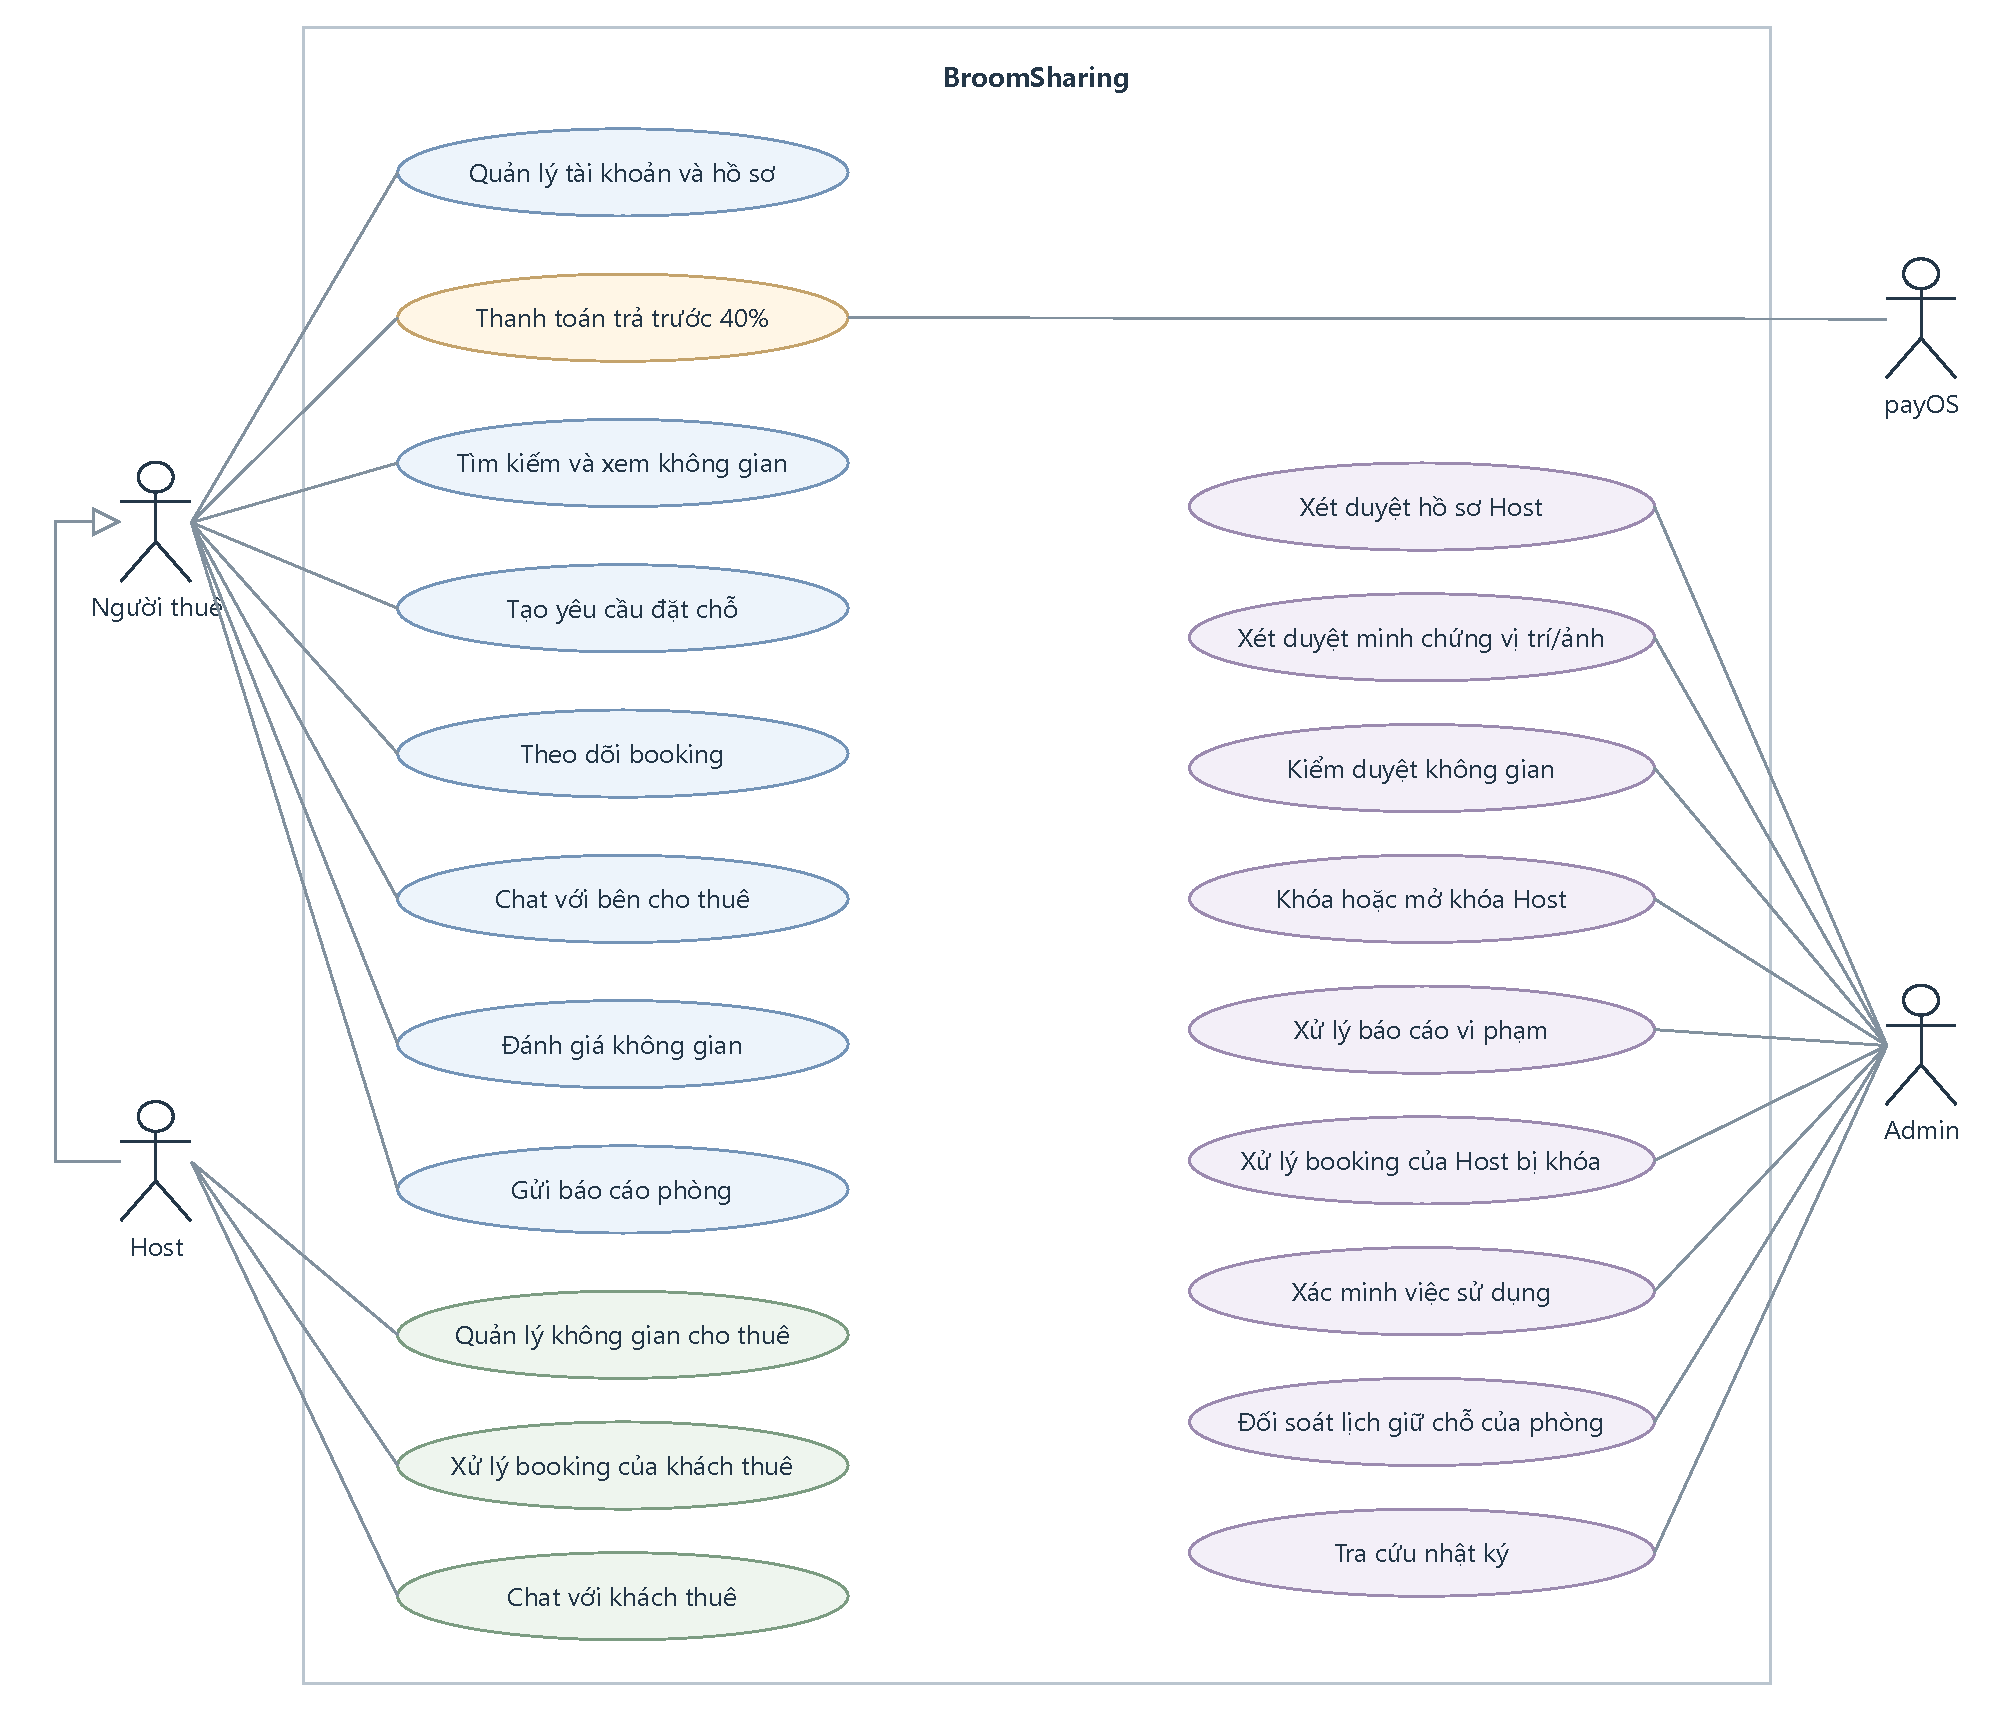
\includegraphics[page=1,width=0.95\textwidth]{chapter2/usecase_diagram_v2.pdf}
\caption{Use case tổng quát với các tác nhân người thuê, Host, Admin và dịch vụ thanh toán.}\label{fig:ch2-usecase-overview}
\end{figure}

Ở phân hệ người thuê, đặt chỗ luôn bao gồm kiểm tra khả dụng và mở bước thanh toán, còn hủy booking là thao tác có điều kiện trên lượt đang được theo dõi. Gửi đơn làm Host bao gồm cung cấp hai ảnh DEMO. Các phân hệ Host và Admin giữ liên kết tác nhân với mục tiêu nghiệp vụ; những cập nhật lịch và nhật ký được mô tả trong quy trình xử lý. Hình~\ref{fig:app-usecase-guest}, Hình~\ref{fig:app-usecase-host} và Hình~\ref{fig:app-usecase-admin} trình bày chi tiết mục tiêu của từng phân hệ.


Phân hệ người thuê bao quát truy cập tài khoản, khám phá, đặt chỗ và tương tác sau thuê. Kiểm tra khả dụng và mở thanh toán thuộc thao tác đặt chỗ; hủy booking chỉ thực hiện khi lượt thuê còn đáp ứng điều kiện hủy.
\begin{figure}[H]\centering
\includegraphics[page=2,width=\textwidth,height=0.75\textheight,keepaspectratio]{chapter2/usecase_diagram_v2.pdf}
\caption{Use case chi tiết của người thuê.}\label{fig:app-usecase-guest}
\end{figure}
Host quản lý tài sản, lịch và việc thực hiện lượt thuê; Admin xét duyệt, xử lý vi phạm và can thiệp booking trong phạm vi quản trị. Hình~\ref{fig:app-usecase-host} và Hình~\ref{fig:app-usecase-admin} thể hiện hai nhóm mục tiêu này. Quyền thuê chung của Host được kế thừa ở sơ đồ tổng quát; xác minh sử dụng và đối soát lịch là các mục tiêu quản trị riêng.

\begin{figure}[H]\centering
\begin{minipage}[t]{0.485\textwidth}\vspace{0pt}\centering
\includegraphics[page=3,width=\linewidth,height=0.67\textheight,keepaspectratio]{chapter2/usecase_diagram_v2.pdf}
\caption{Use case chi tiết của Host.}\label{fig:app-usecase-host}
\end{minipage}\hfill
\begin{minipage}[t]{0.485\textwidth}\vspace{0pt}\centering
\includegraphics[page=4,width=\linewidth,height=0.67\textheight,keepaspectratio]{chapter2/usecase_diagram_v2.pdf}
\caption{Use case chi tiết của Admin.}\label{fig:app-usecase-admin}
\end{minipage}
\end{figure}

\subsection{Ràng buộc nghiệp vụ và yêu cầu phi chức năng}
Các workflow trên chịu những ràng buộc tại Bảng~\ref{tab:ch2-constraints}. Mỗi thao tác được kiểm tra lại từ trạng thái hiện tại và quyền của người thực hiện; việc ẩn hoặc hiện nút trên màn hình không thay thế kiểm tra tại tầng dữ liệu.

\begin{table}[H]\centering\small
\caption{Các ràng buộc thiết kế chính}\label{tab:ch2-constraints}
\begin{tabularx}{\linewidth}{@{}p{3.2cm}X@{}}\toprule
Nhóm & Ràng buộc\\\midrule
Hình thức thuê & Mỗi phòng dùng HOURLY hoặc FIXED; FIXED thuê một hoặc ba tháng. Host chỉ đổi cấu hình khi không còn booking giữ chỗ.\\
Chống đặt trùng & Kiểm tra lại phòng và lịch trong transaction. Cùng request ID và nội dung trả lại booking đã tạo, tránh sinh lượt thuê lặp.\\
Giữ chỗ và tiền & PENDING tạm giữ tối đa 5 phút, không vượt giờ bắt đầu. Đủ 40\% đúng hạn mới xác nhận; quá hạn chưa trả thì nhả lịch, giữ lịch sử.\\
Khép lượt thuê & Xác minh sử dụng trước khi hoàn tất hoặc cho đánh giá; hủy, hết hạn hay kết thúc do sự cố phải nhả đúng khóa lịch, không thực hiện hai lần.\\
Quản trị & Khóa Host hoặc đình chỉ phòng ngăn nhận đặt mới, không xóa lịch sử. Gỡ đình chỉ đưa phòng về không hoạt động để Host kiểm tra trước khi mở lại.\\
Phân quyền & Kiểm tra UID, vai trò và quan hệ sở hữu tại Rules; backend thanh toán xác thực danh tính và lấy số tiền từ dữ liệu đã chốt \parencite{firebase_rules_conditions}.\\
Phản hồi giao diện & Phân biệt đang tải, trống, lỗi và thành công; giữ dữ liệu biểu mẫu phù hợp, nhận cập nhật và cho phép thử lại khi có lỗi kết nối.\\
\bottomrule\end{tabularx}
\end{table}

Báo cáo vi phạm và đánh giá có mục đích riêng: báo cáo chuyển tới Admin để xử lý, còn đánh giá phản ánh một lượt đã sử dụng. Việc can thiệp booking của Host bị khóa được thực hiện từng trường hợp và lưu lý do, không tự suy ra đã thu hoặc hoàn tiền.
